% RQ3 design: the four tumour-dependence analyses. Included from sections/methods.tex.
% Source: figures/figure4/rq3_design_fig.tex (build commands in its header).
\begin{figure}[!htbp]
\centering
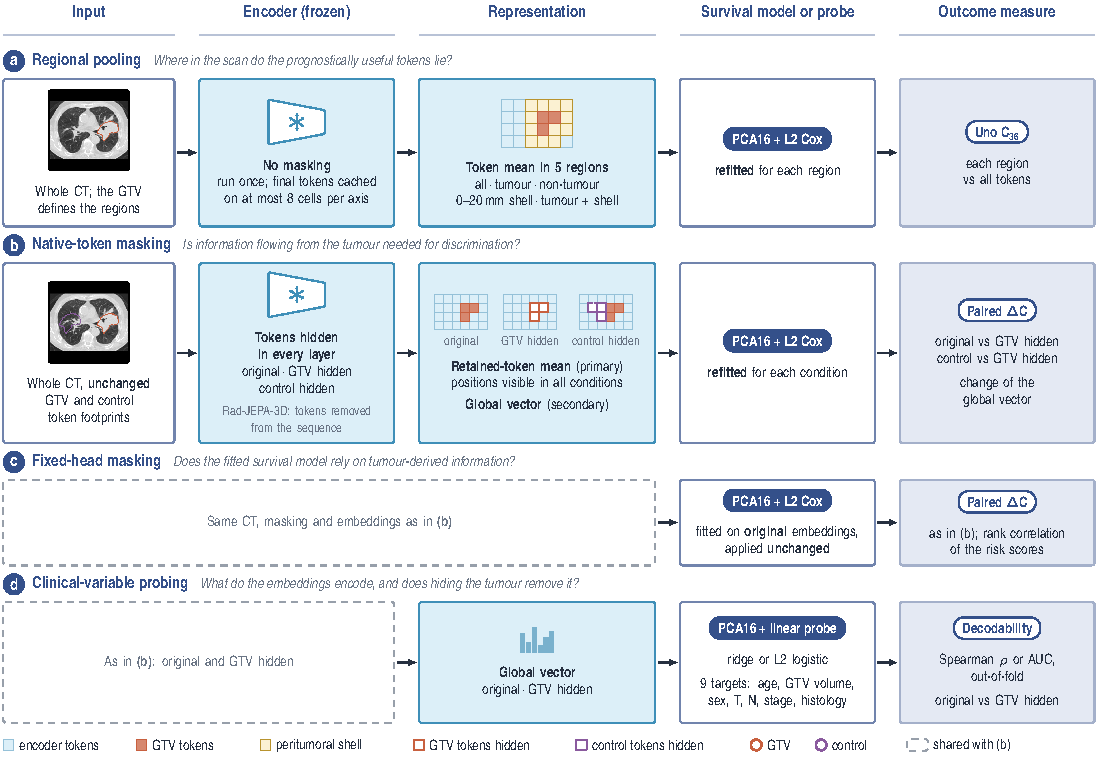
\includegraphics[width=\linewidth]{figures/rq3_design.pdf}
\caption{Design of the four tumour-dependence analyses (RQ3). Each row shows the input, the frozen encoder, the representation, the survival model or probe and the outcome measure. All survival models and probes were fitted on the development folds, with penalties selected by three-fold inner cross-validation, and evaluated on the same five outer test folds. (a) Regional pooling pools the cached final tokens of the unmasked encoder over regions defined by the primary tumour (GTV). (b) Native-token masking leaves the CT unchanged and hides, in every layer of the encoder, the native tokens that contain a GTV voxel, or the same number of tokens around the GTV shape translated within the same axial level (control). Each CT is encoded three times: original, GTV hidden and control hidden. In all three, the primary representation averages the tokens at the same positions, outside both the GTV and the control region, so the conditions differ only in what these tokens received from the hidden region inside the encoder. (c) Fixed-head masking uses the embeddings of (b) but does not refit the survival model. (d) Probing decodes clinical variables from the global vector, with and without the tumour hidden. The CT slice (LUNG1-001) and the control outline are illustrative; grid icons show a single axial level, whereas pooling and masking were applied to the three-dimensional token grid.}
\label{fig:rq3design}
\end{figure}
